%==============================================================================
%  OpenShieldHIT — Parallelisation strategies & memory access
%  Discussion deck (Leszek Grzanka / Niels Bassler)
%
%  Build:  pdflatex slides.tex   (run twice for the section TOC / page refs)
%  Needs:  beamer, tikz, pgfplots  (texlive-latex-recommended + texlive-pictures)
%
%  Every diagram is grounded in the actual code base:
%    - struct osh_rng                 src/random/osh_rng.h
%    - osh_rng_seed_history / split   src/random/osh_rng.h
%    - struct osh_particle_pool (SoA) src/common/osh_particle_pool.h
%    - cold -> hot workspaces         docs/dev/architecture.md
%    - BDO merge / per-thread pages   src/scoring/README.md
%    - host detection + mem budget    src/apps/osh/osh_membudget.*  (#152/#153)
%==============================================================================
\documentclass[aspectratio=169,10pt]{beamer}

\usetheme{default}
\usecolortheme{seahorse}
\setbeamertemplate{navigation symbols}{}
\setbeamertemplate{footline}[frame number]
\useinnertheme{rectangles}

\usepackage{tikz}
\usepackage{pgfplots}
\pgfplotsset{compat=1.16}
\usetikzlibrary{arrows.meta,positioning,fit,backgrounds,calc,shapes.geometric,
                decorations.pathreplacing,shadows.blur,patterns}

\usepackage{lmodern}
\usepackage[T1]{fontenc}

%---- palette ----------------------------------------------------------------
\definecolor{oshBlue}{HTML}{1f4e79}
\definecolor{oshSky}{HTML}{2e86c1}
\definecolor{oshTeal}{HTML}{17a2b8}
\definecolor{oshGreen}{HTML}{2e8b57}
\definecolor{oshAmber}{HTML}{e08e0b}
\definecolor{oshRed}{HTML}{c0392b}
\definecolor{oshGrey}{HTML}{6c757d}
\definecolor{oshLight}{HTML}{eef3f8}
\definecolor{oshPaper}{HTML}{f7f7f5}

\setbeamercolor{frametitle}{fg=white,bg=oshBlue}
\setbeamercolor{title}{fg=oshBlue}
\setbeamercolor{structure}{fg=oshSky}
\setbeamercolor{normal text}{fg=black!88}

%---- reusable tikz styles ---------------------------------------------------
\tikzset{
  >={Stealth[length=2.2mm]},
  box/.style={rounded corners=2pt, draw=oshBlue!70, fill=oshLight,
              align=center, inner sep=4pt, font=\scriptsize},
  shared/.style={rounded corners=2pt, draw=oshGreen!75, fill=oshGreen!12,
              align=center, inner sep=4pt, font=\scriptsize},
  private/.style={rounded corners=2pt, draw=oshAmber!85, fill=oshAmber!14,
              align=center, inner sep=4pt, font=\scriptsize},
  hot/.style={rounded corners=2pt, draw=oshRed!80, fill=oshRed!12,
              align=center, inner sep=4pt, font=\scriptsize},
  worker/.style={rounded corners=3pt, draw=oshSky!80, fill=white,
              align=center, inner sep=5pt, font=\scriptsize, blur shadow={shadow blur steps=4}},
  cell/.style={draw=oshGrey!60, minimum width=7mm, minimum height=6mm,
              font=\tiny, inner sep=1pt},
  lbl/.style={font=\scriptsize\itshape, text=oshGrey},
  ann/.style={font=\scriptsize, text=oshBlue},
  flow/.style={->, draw=oshBlue!75, line width=0.9pt},
  cflow/.style={->, draw=oshGreen!70, line width=0.9pt},
  reduce/.style={->, draw=oshAmber!85, line width=1.0pt, dashed},
}

\newcommand{\code}[1]{{\ttfamily\footnotesize #1}}
\newcommand{\shared}{\tikz\node[shared,inner sep=2pt]{};}
\newcommand{\sprivate}{\tikz\node[private,inner sep=2pt]{};}

\title{Parallelisation strategies for OpenShieldHIT}
\subtitle{Where the histories go, and where the memory lives}
\author{Leszek Grzanka \and Niels Bassler}
\date{Discussion deck — \today}

%==============================================================================
\begin{document}

\begin{frame}[plain]
  \titlepage
  \begin{center}\scriptsize\color{oshGrey}
    Monte Carlo particle transport in C \;$\cdot$\; hardware-aware by design
  \end{center}
\end{frame}

%------------------------------------------------------------------------------
\begin{frame}{The shape of the problem}
  \begin{columns}[T]
    \begin{column}{0.54\textwidth}
      \small
      A Monte Carlo run is \textbf{$N$ independent histories}.
      \medskip

      \textbf{Compute} is embarrassingly parallel: each history is a private
      random walk through the geometry.

      \medskip
      The hard parts are \textbf{not} the physics — they are:
      \begin{itemize}
        \item \textbf{Reproducibility} — same answer regardless of thread / rank / batch?
        \item \textbf{Scoring} — many histories write the \emph{same} voxels.
        \item \textbf{Memory} — what is \textcolor{oshGreen}{shared \& read-only}
              vs.\ \textcolor{oshAmber}{private \& written}.
      \end{itemize}
      \medskip
      This deck walks four strategies and the memory-access pattern of each.
    \end{column}
    \begin{column}{0.46\textwidth}
      \centering
      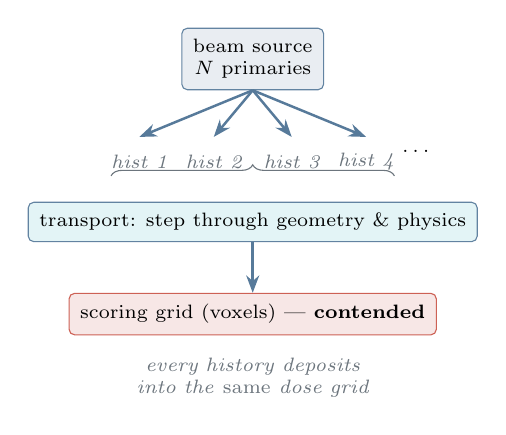
\begin{tikzpicture}[scale=0.9]
        \node[box,fill=oshBlue!10] (src) at (0,3) {beam source\\$N$ primaries};
        \foreach \i/\x in {1/-1.6,2/-0.55,3/0.55,4/1.6}{
          \draw[flow] (src.south) -- (\x,1.9);
          \node[lbl] at (\x,1.55) {hist \i};
        }
        \node at (2.3,1.7) {\scriptsize $\dots$};
        \draw[decorate,decoration={brace,amplitude=4pt},oshGrey]
              (-2.0,1.35) -- (2.0,1.35);
        \node[box,fill=oshTeal!12,minimum width=4.6cm] (geo) at (0,0.7)
              {transport: step through geometry \& physics};
        \node[hot,minimum width=4.6cm] (sc) at (0,-0.6)
              {scoring grid (voxels) — \textbf{contended}};
        \draw[flow] (geo) -- (sc);
        \node[lbl,text width=4.4cm,align=center] at (0,-1.5)
              {every history deposits into the \emph{same} dose grid};
      \end{tikzpicture}
    \end{column}
  \end{columns}
\end{frame}

%------------------------------------------------------------------------------
\begin{frame}{Architecture already built for it: cold $\to$ hot}
  \begin{columns}[T]
    \begin{column}{0.46\textwidth}
      \small
      The app layer parses files into \textbf{four cold workspaces}, then
      \code{*\_prepare()} compiles them into immutable runtime state.

      \medskip
      \textbf{Key for parallelism:} once prepared, the
      \textcolor{oshGreen}{cold/compiled state is read-only}. It can be
      \emph{shared} by every worker with zero coordination.

      \medskip
      Only the \textcolor{oshAmber}{hot, per-history state} (RNG, particle
      pool, scoring tallies) needs a parallel story.
    \end{column}
    \begin{column}{0.54\textwidth}
      \centering
      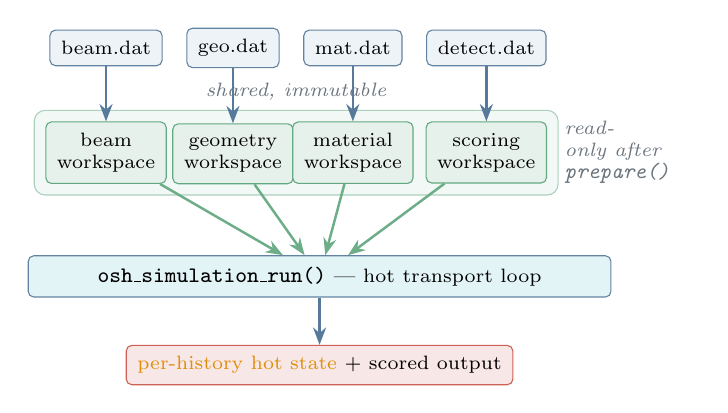
\begin{tikzpicture}[node distance=3mm]
        \node[box] (b) {beam.dat};
        \node[box,right=of b] (g) {geo.dat};
        \node[box,right=of g] (m) {mat.dat};
        \node[box,right=of m] (d) {detect.dat};
        \node[shared,below=7mm of b] (bw){beam\\workspace};
        \node[shared,below=7mm of g] (gw){geometry\\workspace};
        \node[shared,below=7mm of m] (mw){material\\workspace};
        \node[shared,below=7mm of d] (dw){scoring\\workspace};
        \foreach \a/\c in {b/bw,g/gw,m/mw,d/dw}{\draw[flow](\a)--(\c);}
        \node[lbl,right=1mm of dw,text width=1.6cm] {\scriptsize read-only after \code{prepare()}};
        \node[box,fill=oshTeal!12,minimum width=7.4cm,below=9mm of gw.south,
              anchor=north,xshift=1.1cm] (sim)
              {\code{osh\_simulation\_run()} — hot transport loop};
        \foreach \c in {bw,gw,mw,dw}{\draw[cflow](\c)--(sim);}
        \node[hot,below=6mm of sim] (out){\textcolor{oshAmber}{per-history hot state} +
              scored output};
        \draw[flow](sim)--(out);
        \begin{scope}[on background layer]
          \node[fit=(bw)(dw),rounded corners,fill=oshGreen!6,draw=oshGreen!40,
                inner sep=4pt,label={[lbl]above:shared, immutable}]{};
        \end{scope}
      \end{tikzpicture}
    \end{column}
  \end{columns}
  \vspace{1mm}
  \footnotesize\color{oshGrey}
  Source: \code{docs/dev/architecture.md} — four cold workspaces, library never touches files.
\end{frame}

%------------------------------------------------------------------------------
\begin{frame}{The foundation: per-history RNG streams}
  \begin{columns}[T]
    \begin{column}{0.5\textwidth}
      \small
      Reproducibility is decided \emph{before} any thread exists.

      \smallskip
      \code{osh\_rng\_seed\_history(rng, type, seed,\\ hist\_index, purpose)}
      mixes the key through SplitMix64 — the stream depends \textbf{only on
      its key}, never on execution order.
      \begin{itemize}\itemsep1pt
        \item Same history $\Rightarrow$ same draws on any thread, rank, or pool size.
        \item Rank $r$ owns \code{[hist\_base + r$\cdot$N, \dots)} — disjoint,
              non-overlapping streams $\Rightarrow$ MPI splitting is trivial.
        \item Secondaries get \code{osh\_rng\_split()} from the parent —
              independent of scheduling.
        \item \code{struct osh\_rng} is 56\,B, pointer-free $\Rightarrow$
              copies to a GPU slot trivially.
      \end{itemize}
    \end{column}
    \begin{column}{0.5\textwidth}
      \centering
      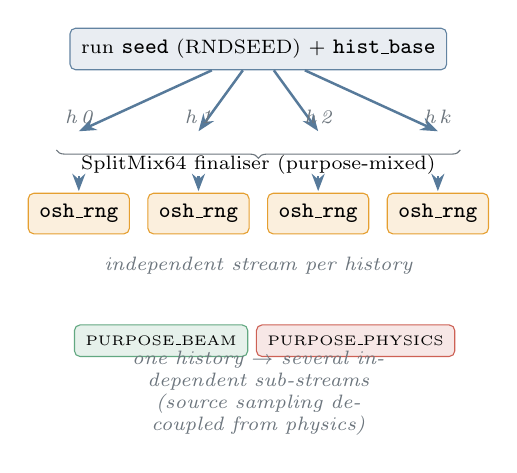
\begin{tikzpicture}[scale=0.95]
        \node[box,fill=oshBlue!10] (seed) at (0,3.1) {run \code{seed} (RNDSEED) + \code{hist\_base}};
        \foreach \i/\x in {0/-2.4,1/-0.8,2/0.8,k/2.4}{
          \draw[flow] (seed) -- (\x,2.0);
        }
        \foreach \i/\x in {0/-2.4,1/-0.8,2/0.8}{
          \node[lbl] at (\x,2.2) {h\,\i};}
        \node[lbl] at (2.4,2.2){h\,$k$};
        \node[font=\scriptsize] at (0,1.55) {SplitMix64 finaliser (purpose-mixed)};
        \draw[decorate,decoration={brace,mirror,amplitude=3pt},oshGrey](-2.7,1.75)--(2.7,1.75);
        \foreach \x in {-2.4,-0.8,0.8,2.4}{
          \node[private,minimum width=1.0cm] at (\x,0.9) {\code{osh\_rng}};
          \draw[flow] (\x,1.4) -- (\x,1.2);}
        \node[lbl] at (0,0.2) {independent stream per history};
        % purposes
        \node[shared,minimum width=2.0cm,font=\tiny] (bm) at (-1.3,-0.8){PURPOSE\_BEAM};
        \node[hot,minimum width=2.0cm,font=\tiny] (ph) at (1.3,-0.8){PURPOSE\_PHYSICS};
        \node[lbl,text width=5cm,align=center] at (0,-1.5)
              {one history $\to$ several independent sub-streams\\(source sampling decoupled from physics)};
      \end{tikzpicture}
    \end{column}
  \end{columns}
  \vspace{0.5mm}
  \footnotesize\color{oshGrey}
  Source: \code{src/random/osh\_rng.h} — \code{osh\_rng\_seeding}, \code{osh\_rng\_seed\_history}, \code{osh\_rng\_split}.
\end{frame}

%------------------------------------------------------------------------------
\section{Strategies}
\begin{frame}{Four strategies on one axis}
  \centering
  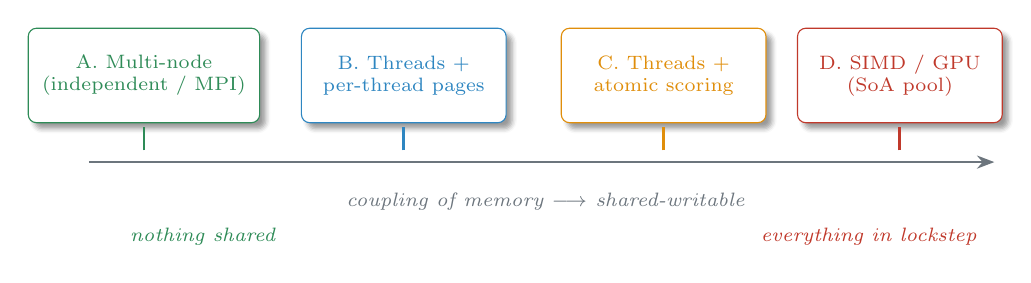
\begin{tikzpicture}[scale=1.0]
    \draw[->,oshGrey,line width=1pt] (-0.3,0) -- (11.2,0);
    \node[lbl] at (5.5,-0.5) {coupling of memory $\longrightarrow$ shared-writable};
    \foreach \x/\name/\col in {0.4/{A. Multi-node\\(independent / MPI)}/oshGreen,
                               3.7/{B. Threads +\\per-thread pages}/oshSky,
                               7.0/{C. Threads +\\atomic scoring}/oshAmber,
                               10.0/{D. SIMD / GPU\\(SoA pool)}/oshRed}{
      \node[worker,draw=\col,minimum width=2.6cm,minimum height=1.2cm,
            font=\scriptsize,text=\col] at (\x,1.1) {\name};
      \draw[\col,line width=1pt] (\x,0.15)--(\x,0.45);
    }
    \node[lbl,text=oshGreen,anchor=west] at (0.1,-0.95) {nothing shared};
    \node[lbl,text=oshRed,anchor=east] at (11.1,-0.95) {everything in lockstep};
  \end{tikzpicture}
  \vspace{2mm}
  \begin{itemize}\small
    \item Moving right: \textbf{less memory}, \textbf{more contention}, \textbf{harder reproducibility}.
    \item They compose: e.g.\ \textbf{MPI across nodes} $\times$ \textbf{threads within a node} $\times$ \textbf{SIMD within a thread}.
  \end{itemize}
\end{frame}

%------------------------------------------------------------------------------
\begin{frame}{Strategy A — Multi-node / embarrassingly parallel}
  \begin{columns}[T]
    \begin{column}{0.46\textwidth}
      \small
      Each process is a \textbf{full, independent run} over a disjoint
      history range. Nothing is shared at runtime.
      \begin{itemize}\itemsep2pt
        \item Memory: every rank holds its \emph{own} copy of geometry +
              scoring grid.
        \item Communication: \textbf{none} until the end.
        \item Merge \code{.bdo} files; each carries its own \code{nstat}.
      \end{itemize}
      \textbf{Per-scorer merge rule} (scoring README):
      \begin{itemize}\scriptsize\itemsep1pt
        \item NORM (DOSE\dots): $\;X=\frac{\sum_j x_j}{\sum_j \mathrm{nstat}_j}$
        \item AVER (DLET\dots): $\;X=\frac{\sum_j x_j\,\mathrm{nstat}_j}{\sum_j \mathrm{nstat}_j}$
        \item SUM (COUNT): $\;X=\sum_j x_j$ \quad APPEND (MCPL): concat
      \end{itemize}
      \textcolor{oshGreen}{$+$} trivial, near-linear, robust.\quad
      \textcolor{oshRed}{$-$} grid replicated per rank.
    \end{column}
    \begin{column}{0.54\textwidth}
      \centering
      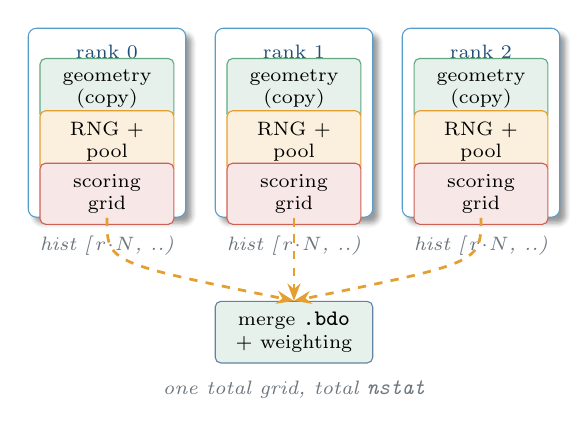
\begin{tikzpicture}[scale=0.95]
        \foreach \r/\x in {0/0,1/2.5,2/5.0}{
          \node[worker,minimum width=2.0cm,minimum height=2.4cm] (w\r) at (\x,1.6) {};
          \node[ann] at (\x,2.55) {rank \r};
          \node[shared,minimum width=1.7cm] at (\x,2.05) {geometry\\(copy)};
          \node[private,minimum width=1.7cm] at (\x,1.35) {RNG +\\pool};
          \node[hot,minimum width=1.7cm] at (\x,0.65) {scoring\\grid};
          \node[lbl] at (\x,-0.05) {hist [\,$r\!\cdot\!N$, ..)};
        }
        \node[box,fill=oshGreen!12,minimum width=2.0cm] (m) at (2.5,-1.2) {merge \code{.bdo}\\$+$ weighting};
        \foreach \r in {0,1,2}{\draw[reduce] (w\r.south) .. controls +(0,-0.6) .. (m.north);}
        \node[lbl,below=1mm of m] {one total grid, total \code{nstat}};
      \end{tikzpicture}
    \end{column}
  \end{columns}
\end{frame}

%------------------------------------------------------------------------------
\begin{frame}{Strategy B — Threads + per-thread scoring pages}
  \begin{columns}[T]
    \begin{column}{0.46\textwidth}
      \small
      One process, $T$ threads. Geometry \& material are
      \textcolor{oshGreen}{shared read-only}; each thread owns a
      \textcolor{oshAmber}{private particle pool and private scoring pages}.
      \begin{itemize}\itemsep2pt
        \item No write contention during transport.
        \item One \textbf{reduction} (sum the per-thread pages) at the end,
              then write a single \code{.bdo}.
        \item This is the ``native multi-threaded'' path the scoring layer is
              already designed for.
      \end{itemize}
      \textcolor{oshGreen}{$+$} no atomics, cache-friendly, deterministic
      reduction.\\
      \textcolor{oshRed}{$-$} scoring memory $\times\,T$ (matters for large grids).
    \end{column}
    \begin{column}{0.54\textwidth}
      \centering
      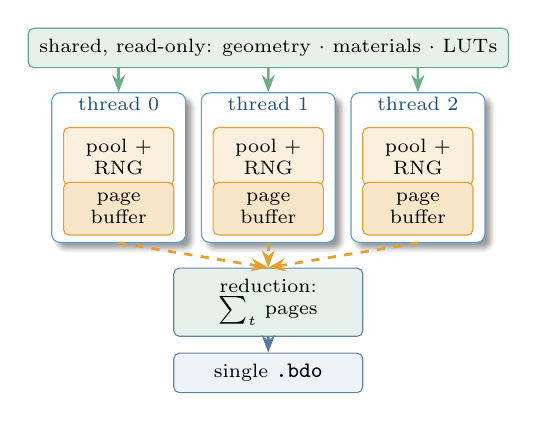
\begin{tikzpicture}[scale=0.95]
        \node[shared,minimum width=4.8cm] (geo) at (2.0,3.0)
              {shared, read-only: geometry $\cdot$ materials $\cdot$ LUTs};
        \foreach \t/\x in {0/0,1/2.0,2/4.0}{
          \node[worker,minimum width=1.7cm,minimum height=1.9cm] (t\t) at (\x,1.4){};
          \node[ann] at (\x,2.25){thread \t};
          \node[private,minimum width=1.4cm] at (\x,1.55){pool +\\RNG};
          \node[private,minimum width=1.4cm,fill=oshAmber!22] at (\x,0.85){page\\buffer};
          \draw[cflow] (geo.south-|\x,0) -- (t\t.north);
        }
        \node[box,fill=oshGreen!12,minimum width=2.4cm] (red) at (2.0,-0.4)
              {reduction:\\$\sum_t$ pages};
        \foreach \t in {0,1,2}{\draw[reduce](t\t.south)--(red.north);}
        \node[box,minimum width=2.4cm,below=2mm of red](bdo){single \code{.bdo}};
        \draw[flow](red)--(bdo);
      \end{tikzpicture}
    \end{column}
  \end{columns}
  \vspace{0.5mm}
  \footnotesize\color{oshGrey}
  Source: \code{src/scoring/README.md} (per-thread pages, summed by simulation layer);
  \code{osh\_particle\_pool.h} (one pool per thread).
\end{frame}

%------------------------------------------------------------------------------
\begin{frame}{Strategy C — Threads + atomic scoring (the contrast)}
  \begin{columns}[T]
    \begin{column}{0.46\textwidth}
      \small
      Threads share \emph{one} scoring grid and update it with atomics.
      Saves the $\times T$ memory of Strategy B — but pays at the hardware level.
      \begin{itemize}\itemsep2pt
        \item \textbf{Contention} on hot voxels (Bragg peak!) — many threads,
              one cache line.
        \item \textbf{False sharing}: neighbouring voxels in the same 64\,B
              line ping-pong between cores even when logically disjoint.
        \item Atomic add on \code{double} $\Rightarrow$ summation order varies
              $\Rightarrow$ not bit-identical (physics still correct).
      \end{itemize}
      \textcolor{oshGreen}{$+$} O(1) scoring memory.\quad
      \textcolor{oshRed}{$-$} cache-line warfare on the peak.
    \end{column}
    \begin{column}{0.54\textwidth}
      \centering
      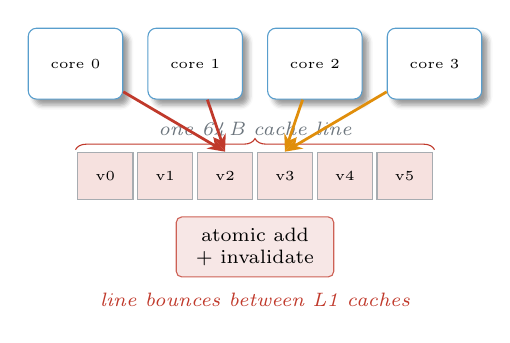
\begin{tikzpicture}[scale=0.95]
        \foreach \t/\x in {0/0,1/1.6,2/3.2,3/4.8}{
          \node[worker,minimum width=1.2cm,minimum height=0.9cm,font=\tiny] (c\t) at (\x,3.0){core \t};
        }
        % cache line of voxels
        \node[lbl] at (2.4,2.1){one 64\,B cache line};
        \foreach \i/\x in {0/0.4,1/1.2,2/2.0,3/2.8,4/3.6,5/4.4}{
          \node[cell,fill=oshRed!15] (v\i) at (\x,1.5){v\i};
        }
        \draw[decorate,decoration={brace,amplitude=4pt},oshRed](0.0,1.85)--(4.8,1.85);
        % collisions
        \draw[->,oshRed,line width=1pt] (c0) -- (v2.north);
        \draw[->,oshRed,line width=1pt] (c1) -- (v2.north);
        \draw[->,oshAmber,line width=1pt] (c2) -- (v3.north);
        \draw[->,oshAmber,line width=1pt] (c3) -- (v3.north);
        \node[hot,minimum width=2.0cm] at (2.4,0.55){atomic add\\+ invalidate};
        \node[lbl,text=oshRed] at (2.4,-0.15){line bounces between L1 caches};
      \end{tikzpicture}
    \end{column}
  \end{columns}
\end{frame}

%------------------------------------------------------------------------------
\begin{frame}{Strategy D — SIMD / GPU and the SoA pool}
  \begin{columns}[T]
    \begin{column}{0.47\textwidth}
      \small
      The particle pool is \textbf{structure-of-arrays} on purpose: one field,
      all $N$ particles, contiguous $\Rightarrow$ auto-vectorises with no
      gather/scatter.
      \medskip

      \textbf{Batch size = the cache/parallelism dial} (\code{osh\_particle\_pool.h}):
      \begin{itemize}\scriptsize\itemsep1pt
        \item \code{capacity == NSTAT}: all primaries live $\Rightarrow$ max
              parallelism, natural for GPU.
        \item \code{4096..65536}: pool fits L2/L3 $\Rightarrow$ optimal CPU SIMD;
              outer loop $\lceil N/\text{cap}\rceil$ times.
        \item \code{capacity == 1}: scalar serial reference.
      \end{itemize}
      \medskip
      Per-slot \code{osh\_rng} travels \emph{with} the particle, so draws follow
      the history, not the wavefront.\\
      \textcolor{oshRed}{$-$} divergence: histories step/die at different rates.
    \end{column}
    \begin{column}{0.53\textwidth}
      \centering
      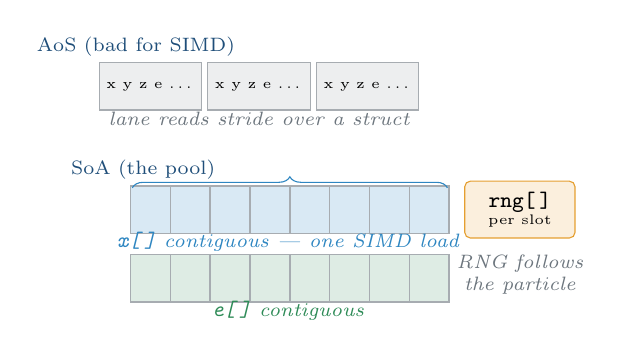
\begin{tikzpicture}[scale=0.92]
        % AoS vs SoA
        \node[ann] at (-0.2,3.25) {AoS (bad for SIMD)};
        \foreach \i/\x in {0/0,1/1.5,2/3.0}{
          \node[cell,minimum width=1.3cm,fill=oshGrey!12] at (\x,2.7){x y z e \dots};}
        \node[lbl] at (1.5,2.25){lane reads stride over a struct};

        \node[ann] at (-0.1,1.55) {SoA (the pool)};
        \foreach \x in {0,0.55,1.1,1.65,2.2,2.75,3.3,3.85}{
          \node[cell,minimum width=5mm,fill=oshSky!18] at (\x,1.0){};}
        \node[lbl,text=oshSky] at (1.9,0.55){\code{x[\,]} contiguous — one SIMD load};
        \foreach \x in {0,0.55,1.1,1.65,2.2,2.75,3.3,3.85}{
          \node[cell,minimum width=5mm,fill=oshGreen!16] at (\x,0.05){};}
        \node[lbl,text=oshGreen] at (1.9,-0.4){\code{e[\,]} contiguous};
        % vector lanes
        \draw[decorate,decoration={brace,amplitude=4pt},oshSky](-0.25,1.3)--(4.1,1.3);
        \node[private,minimum width=1.4cm,font=\tiny] at (5.1,1.0){\code{rng[\,]}\\per slot};
        \node[lbl,text width=2cm,align=center] at (5.1,0.1){RNG follows\\the particle};
      \end{tikzpicture}
    \end{column}
  \end{columns}
  \vspace{0.5mm}
  \footnotesize\color{oshGrey}
  Source: \code{src/common/osh\_particle\_pool.h} — SoA rationale, batch-size guidance, per-slot RNG.
\end{frame}

%------------------------------------------------------------------------------
\section{Memory}
\begin{frame}{Memory access — what is shared vs.\ private}
  \centering
  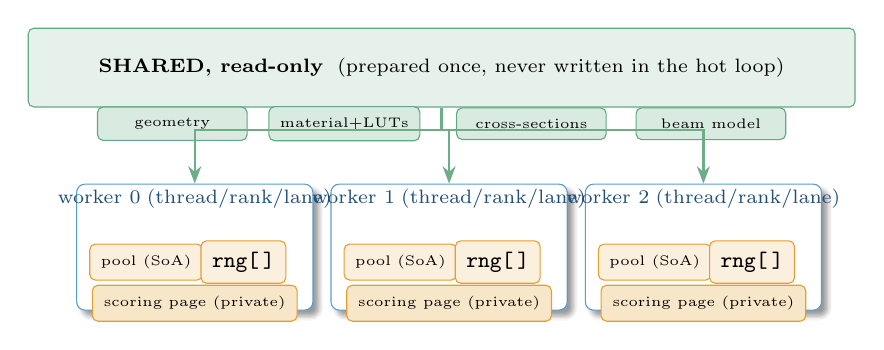
\begin{tikzpicture}[scale=0.95]
    % shared region
    \node[shared,minimum width=10.5cm,minimum height=1.0cm] (sh) at (5,3.3)
          {\textbf{SHARED, read-only} \;(prepared once, never written in the hot loop)};
    \foreach \t/\x in {geometry/1.4, material+LUTs/3.7, cross-sections/6.2, beam model/8.6}{
      \node[shared,fill=oshGreen!18,font=\tiny,minimum width=1.9cm] at (\x,2.55){\t};}
    % per worker private
    \foreach \w/\x in {0/0.7,1/4.1,2/7.5}{
      \node[worker,minimum width=3.0cm,minimum height=1.6cm] (pw\w) at (\x+1.0,0.9){};
      \node[ann] at (\x+1.0,1.55){worker \w \;(thread/rank/lane)};
      \node[private,font=\tiny,minimum width=1.3cm] at (\x+0.35,0.7){pool (SoA)};
      \node[private,font=\tiny,minimum width=1.0cm] at (\x+1.65,0.7){\code{rng[\,]}};
      \node[private,fill=oshAmber!22,font=\tiny,minimum width=2.6cm] at (\x+1.0,0.15){scoring page (private)};
    }
    \draw[cflow](sh.south)--+(0,-0.3) -| (pw0);
    \draw[cflow](sh.south)--+(0,-0.3) -| (pw1);
    \draw[cflow](sh.south)--+(0,-0.3) -| (pw2);
  \end{tikzpicture}
  \begin{itemize}\scriptsize
    \item[\textcolor{oshGreen}{$\blacksquare$}] Shared read-only $\Rightarrow$ lives once in
          L3 / RAM, no coherence traffic, scales for free.
    \item[\textcolor{oshAmber}{$\blacksquare$}] Private writable $\Rightarrow$ no contention;
          cost is the $\times T$ replication you choose to pay (Strategy B vs.\ C).
  \end{itemize}
\end{frame}

%------------------------------------------------------------------------------
\begin{frame}{Memory access — the cache hierarchy view}
  \begin{columns}[T]
    \begin{column}{0.5\textwidth}
      \centering
      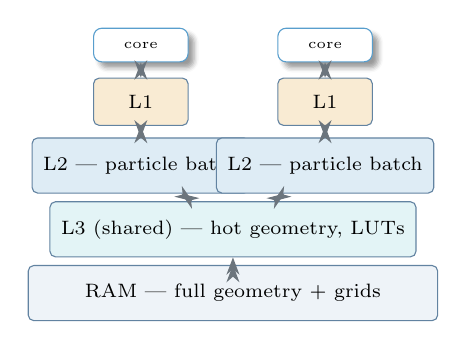
\begin{tikzpicture}[scale=0.9]
        \node[box,fill=oshLight,minimum width=5.2cm,minimum height=0.7cm] (ram) at (0,0){RAM — full geometry + grids};
        \node[box,fill=oshTeal!12,minimum width=4.2cm,minimum height=0.7cm] (l3) at (0,0.9){L3 (shared) — hot geometry, LUTs};
        \node[box,fill=oshSky!16,minimum width=2.7cm,minimum height=0.7cm] (l2) at (-1.3,1.8){L2 — particle batch};
        \node[box,fill=oshSky!16,minimum width=2.7cm,minimum height=0.7cm] (l2b) at (1.3,1.8){L2 — particle batch};
        \node[box,fill=oshAmber!18,minimum width=1.2cm,minimum height=0.6cm] (l1) at (-1.3,2.7){L1};
        \node[box,fill=oshAmber!18,minimum width=1.2cm,minimum height=0.6cm] (l1b) at (1.3,2.7){L1};
        \node[worker,minimum width=1.2cm,font=\tiny] (co) at (-1.3,3.5){core};
        \node[worker,minimum width=1.2cm,font=\tiny] (cob) at (1.3,3.5){core};
        \draw[<->,oshGrey](ram)--(l3);\draw[<->,oshGrey](l3)--(l2);
        \draw[<->,oshGrey](l3)--(l2b);\draw[<->,oshGrey](l2)--(l1);
        \draw[<->,oshGrey](l2b)--(l1b);\draw[<->,oshGrey](l1)--(co);
        \draw[<->,oshGrey](l1b)--(cob);
      \end{tikzpicture}
    \end{column}
    \begin{column}{0.5\textwidth}
      \small
      Design goals that fall out of this picture:
      \begin{itemize}\itemsep3pt
        \item \textbf{Batch to fit L2/L3} (4k--64k particles) so the working
              set stays hot — the pool's documented sweet spot.
        \item \textbf{Share the read-only geometry in L3} — one copy feeds
              all cores.
        \item \textbf{Keep writes in L1-private pages} (Strategy B) to avoid
              cross-core invalidations.
        \item \textbf{Pad / separate hot scorers} to dodge false sharing
              (Strategy C's tax).
        \item Tiny pointer-free \code{osh\_rng} (56\,B) keeps per-lane state in
              registers/L1.
      \end{itemize}
    \end{column}
  \end{columns}
\end{frame}

%------------------------------------------------------------------------------
\begin{frame}{Memory budgeting — already host-aware}
  \begin{columns}[T]
    \begin{column}{0.52\textwidth}
      \small
      Recent work (\#152/\#153) adds \textbf{host detection + memory
      budgeting}: the runtime knows core count and available RAM.
      \medskip

      That is exactly the knob this discussion needs:
      \[
        \underbrace{M_\text{shared}}_{\text{geometry, once}}
        + T\cdot\underbrace{(M_\text{pool}+M_\text{page})}_{\text{per worker}}
        \;\le\; M_\text{host}
      \]
      \begin{itemize}\itemsep2pt
        \item Picks $T$ (threads) and batch capacity to fit the budget.
        \item Decides \textbf{B vs.\ C}: replicate pages while
              $T\cdot M_\text{page}$ fits; switch to atomics when it doesn't.
        \item Bridges naturally to MPI: per-rank budget $\times$ ranks/node.
      \end{itemize}
    \end{column}
    \begin{column}{0.48\textwidth}
      \centering
      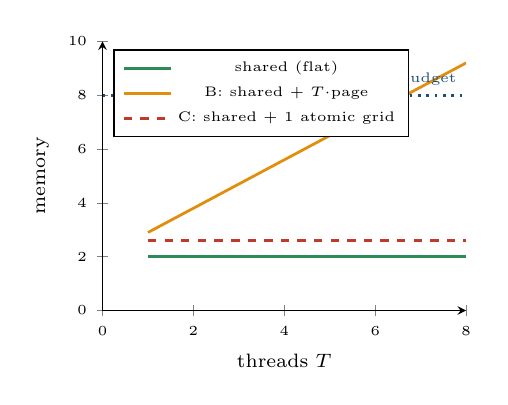
\begin{tikzpicture}
        \begin{axis}[
            width=6.2cm,height=5.0cm,
            xlabel={\scriptsize threads $T$},
            ylabel={\scriptsize memory},
            xmin=0,xmax=8,ymin=0,ymax=10,
            tick label style={font=\tiny},
            label style={font=\scriptsize},
            legend style={font=\tiny,at={(0.03,0.97)},anchor=north west},
            axis lines=left,
          ]
          \addplot[oshGreen,line width=1pt,domain=1:8,samples=8]{2};
          \addlegendentry{shared (flat)}
          \addplot[oshAmber,line width=1pt,domain=1:8,samples=8]{2+0.9*x};
          \addlegendentry{B: shared + $T\cdot$page}
          \addplot[oshRed,dashed,line width=1pt,domain=1:8,samples=8]{2.6};
          \addlegendentry{C: shared + 1 atomic grid}
          \draw[oshBlue,dotted,line width=1pt] (axis cs:0,8)--(axis cs:8,8);
          \node[font=\tiny,oshBlue,anchor=south east] at (axis cs:8,8){host budget};
        \end{axis}
      \end{tikzpicture}
    \end{column}
  \end{columns}
  \vspace{0.5mm}
  \footnotesize\color{oshGrey}
  Source: \code{src/apps/osh/osh\_membudget.*}, \code{src/common/osh\_sysinfo.*} (\#152/\#153).
\end{frame}

%------------------------------------------------------------------------------
\section{Summary}
\begin{frame}{Comparison at a glance}
  \centering
  \renewcommand{\arraystretch}{1.35}
  \footnotesize
  \begin{tabular}{l l l l l l}
    \textbf{Strategy} & \textbf{Shares} & \textbf{Scoring mem} & \textbf{Contention} & \textbf{Repro.} & \textbf{Effort}\\
    \hline
    \textcolor{oshGreen}{A. Multi-node / MPI} & nothing & $\times$ ranks & none & bit-identical$^\ast$ & \textbf{low}\\
    \textcolor{oshSky}{B. Threads + pages} & geo (RO) & $\times T$ & none & deterministic reduce & medium\\
    \textcolor{oshAmber}{C. Threads + atomics} & geo + grid & $\times 1$ & high (peak) & order-dependent & medium\\
    \textcolor{oshRed}{D. SIMD / GPU} & geo (RO) & per lane/block & divergence & per-history stream & high\\
  \end{tabular}
  \vspace{3mm}
  \begin{itemize}\scriptsize
    \item[$\ast$] Per-history streams make A reproducible \emph{by construction}: rank $r$ owns a disjoint history range.
    \item All four sit on the \textbf{same} foundation: read-only cold state + per-history RNG + SoA pool.
  \end{itemize}
\end{frame}

%------------------------------------------------------------------------------
\begin{frame}{A suggested path (for discussion)}
  \centering
  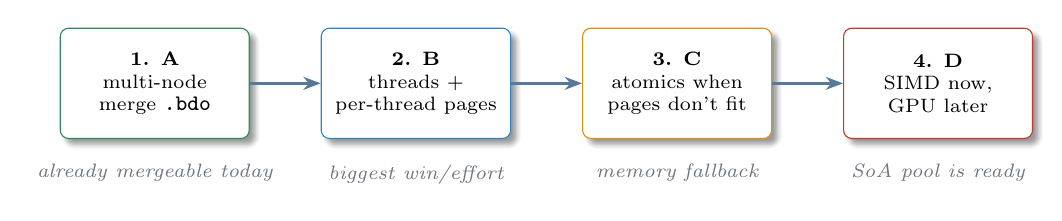
\begin{tikzpicture}[node distance=6mm and 9mm]
    \node[worker,draw=oshGreen,minimum width=2.4cm,minimum height=1.4cm] (a)
         {\textbf{1. A}\\multi-node\\merge \code{.bdo}};
    \node[worker,draw=oshSky,minimum width=2.4cm,minimum height=1.4cm,right=of a] (b)
         {\textbf{2. B}\\threads +\\per-thread pages};
    \node[worker,draw=oshAmber,minimum width=2.4cm,minimum height=1.4cm,right=of b] (c)
         {\textbf{3. C}\\atomics when\\pages don't fit};
    \node[worker,draw=oshRed,minimum width=2.4cm,minimum height=1.4cm,right=of c] (d)
         {\textbf{4. D}\\SIMD now,\\GPU later};
    \draw[flow](a)--(b);\draw[flow](b)--(c);\draw[flow](c)--(d);
    \node[lbl,below=2mm of a]{already mergeable today};
    \node[lbl,below=2mm of b]{biggest win/effort};
    \node[lbl,below=2mm of c]{memory fallback};
    \node[lbl,below=2mm of d]{SoA pool is ready};
  \end{tikzpicture}
  \vspace{4mm}
  \begin{columns}[T]
    \begin{column}{0.5\textwidth}
      \small\textbf{Open questions for the meeting}
      \begin{itemize}\scriptsize\itemsep1pt
        \item Target first: single fat node (B) or cluster (A$\times$B)?
        \item Threading layer: OpenMP vs.\ raw pthreads vs.\ a task pool?
        \item Page reduction: tree-reduce for bit-identity, or atomics?
      \end{itemize}
    \end{column}
    \begin{column}{0.5\textwidth}
      \small\textbf{What is ready vs.\ to build}
      \begin{itemize}\scriptsize\itemsep1pt
        \item \textcolor{oshGreen}{Ready:} per-history RNG, SoA pool, cold/hot split, \code{.bdo} merge rules, mem budget.
        \item \textcolor{oshAmber}{To build:} thread orchestration, per-thread page reduction, MPI history partitioning.
      \end{itemize}
    \end{column}
  \end{columns}
\end{frame}

\begin{frame}[plain]
  \centering
  \vfill
  {\Large\color{oshBlue}\textbf{Discussion}}\\[2mm]
  \small\color{oshGrey}
  Four strategies, one foundation: read-only cold state $\cdot$ per-history RNG $\cdot$ SoA pool.\\
  Diagrams sourced from the OpenShieldHIT code base.
  \vfill
\end{frame}

\end{document}
